Overall the results show that Google Glass is slower than smartphones in all parts of the application. Google Glass performed about half a second slower than the smartphones, where Samsung Galaxy SIII proved to be faster than Samsung Galaxy SII. Using different complexities on the QR code Google Glass was only able to read the QR code encoding one character. Samsung Galaxy SII managed to read the QR code encoding 50 characters, however not the QR code encoding 100 characters. Samsung Galaxy SIII managed to read all three of the QR codes with varying complexity.

Google Glass can also only show somewhere between 200 and 220 characters on screen at the same time, when using a layout design where only text is presented. Using a layout design which displays both text and an image the number of character Google Glass may show on screen is somewhere between 100 and 120.

Since the layout design for the Google Glass application was used as basis for the smartphone application many of the screens in the smartphone application are relatively empty, and could potentially contain much more information.

\subsection{Demo Case}
The result of the implementation is described in the following demonstration case, where the goal is to build a Lego figure, called ``Space Pirate'', seen in Figure~\ref{demoCaseGoal}. The following walkthrough of the demonstration will cover both the Google Glass version as well as the smartphone version. The Lego parts will already be partially assembled in order to reduce the number of slides, as the general idea of the application will still be presented. There are four different components used to assemble the Space Pirate. All of the components can be seen in Figure~\ref{demoCaseRaw}.

	\begin{figure}[H]%ht!]
		\centering
		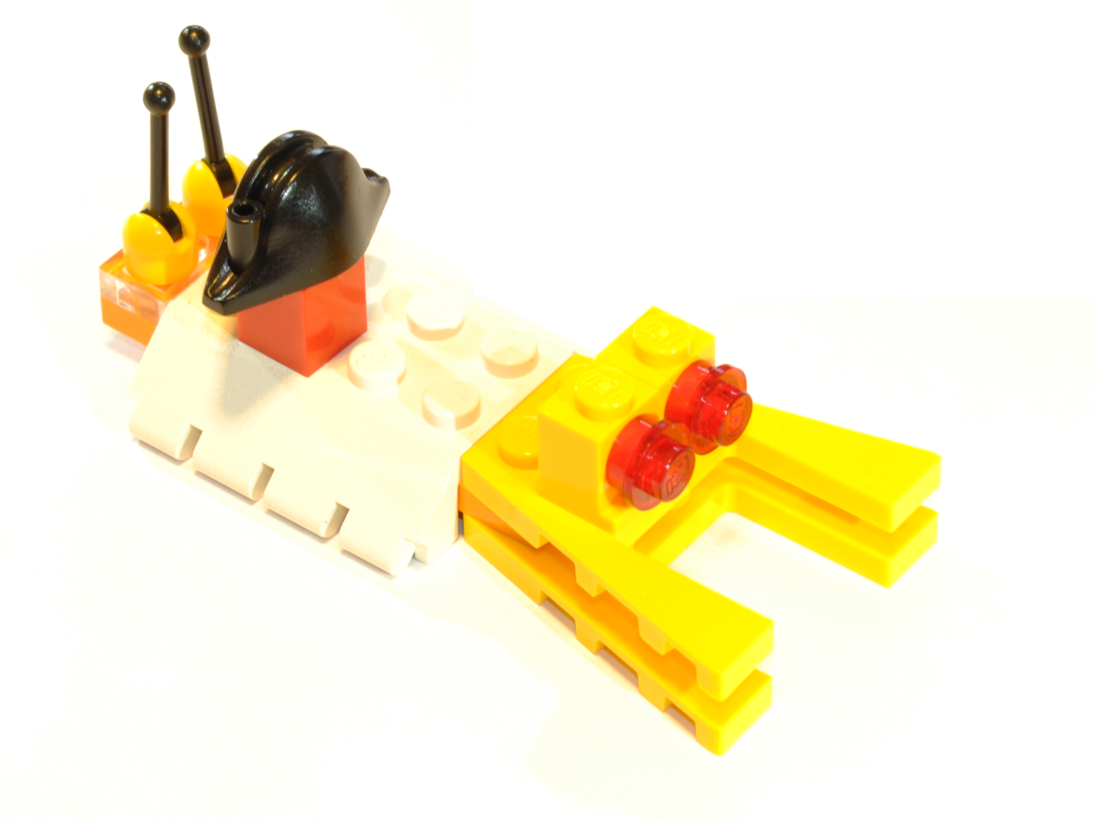
\includegraphics[width=90mm]{images/rawImages/BILD_6}
		\caption{Space Pirate.}
		\label{demoCaseGoal}
	\end{figure}

	\begin{figure}[H]%ht!]
		\centering
		\subfloat[Steering.]{{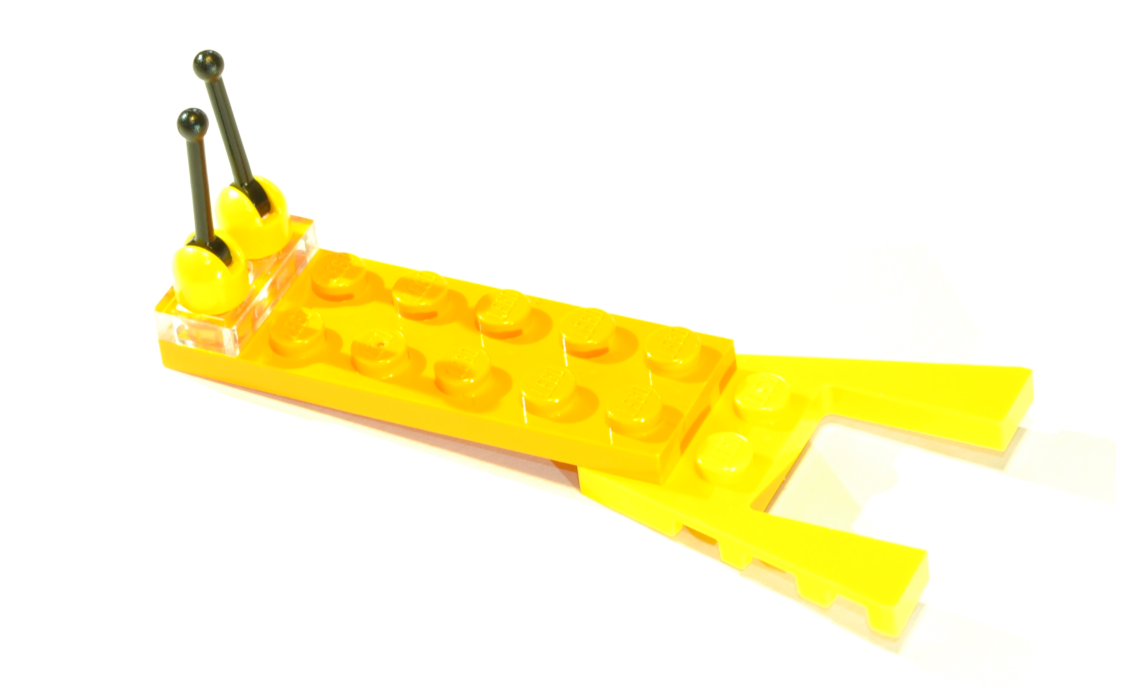
\includegraphics[width=50mm]{images/rawImages/BILD_1}}}
		\qquad
		\subfloat[Tail Light.]{{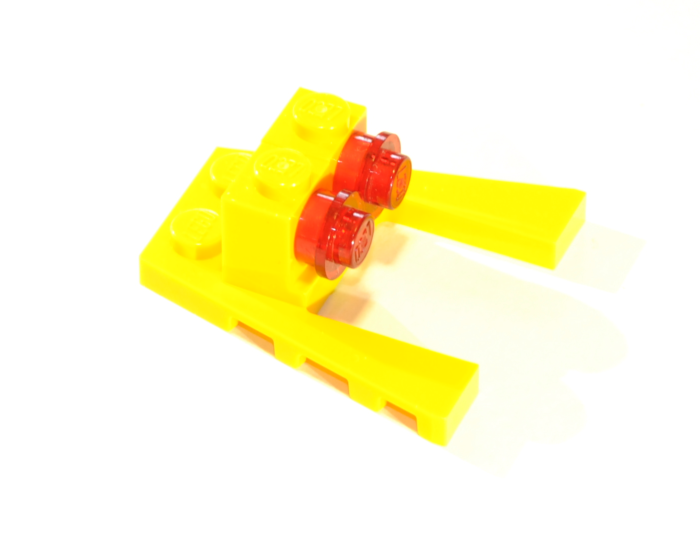
\includegraphics[width=50mm]{images/rawImages/BILD_2}}}
		\qquad
		\subfloat[Body.]{{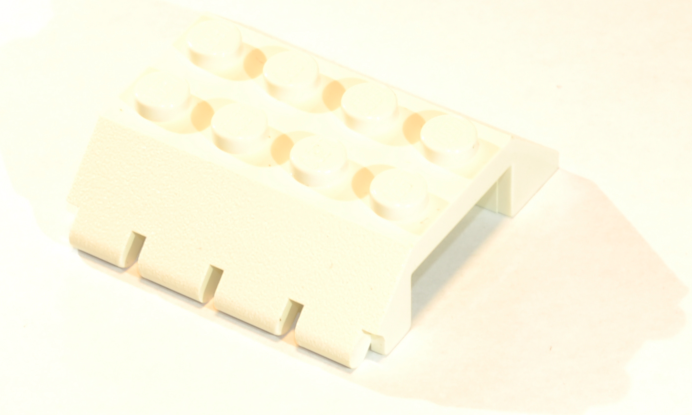
\includegraphics[width=50mm]{images/rawImages/BILD_3}}}
		\qquad
    		\subfloat[Pirate.]{{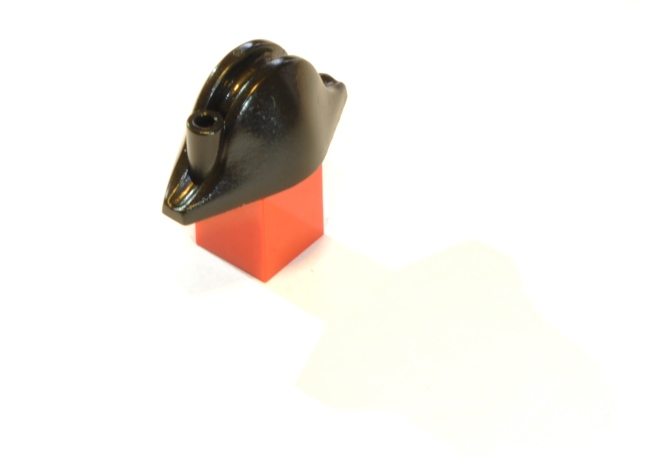
\includegraphics[width=50mm]{images/rawImages/BILD_4}}}
		\qquad
		\caption{Components.}
		\label{demoCaseRaw}
	\end{figure}
\newpage
In order to receive any information on the product the user must scan the product specific QR code, as seen in Figure~\ref{demoCaseQRLoad}~(a) and in Figure~\ref{demoCaseQRLoad}~(c). When the QR code has been scanned the information will be downloaded, as seen in Figure~\ref{demoCaseQRLoad}~(b) and in Figure~\ref{demoCaseQRLoad}~(d).

	\begin{figure}[ht!]
		\centering
		\subfloat[Scanning a QR code in the Google Glass application.]{{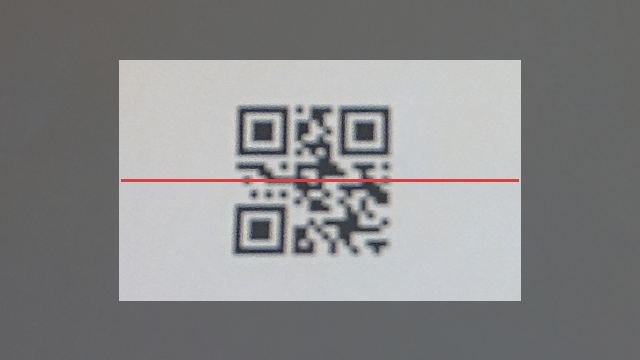
\includegraphics[width=60mm]{images/demo/qrCodeNew}}}
		\qquad
		\subfloat[Loading in the Google Glass application.]{{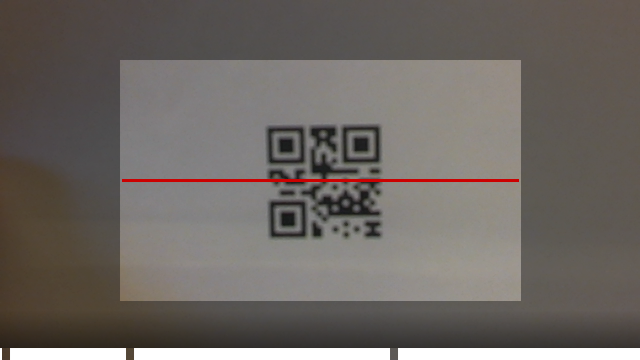
\includegraphics[width=60mm]{images/demo/loadingBar}}}
		\qquad
		\subfloat[Scanning a QR code in the smartphone application.]{{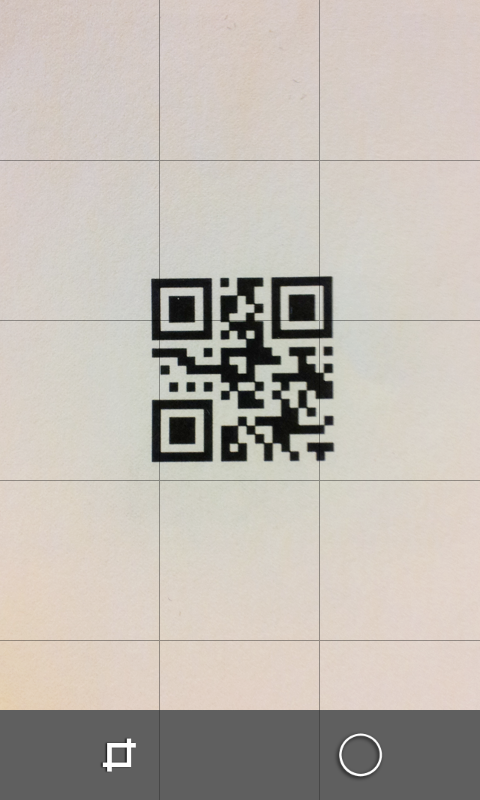
\includegraphics[width=60mm]{images/demo/smartphone/qrCodeNew}}}
		\qquad
    		\subfloat[Loading in the smartphone application.]{{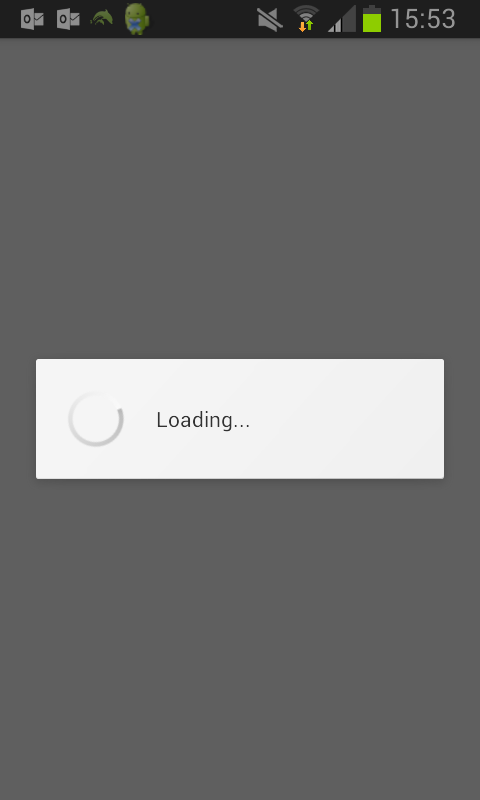
\includegraphics[width=60mm]{images/demo/smartphone/loadingSpinner}}}
		\qquad
		\caption{Scanning and loading screens.}
		\label{demoCaseQRLoad}
	\end{figure}

The first slide the user sees, when the product information has been downloaded and is displayed to the user, is the title slide. The title slide for the Space Pirate can be seen Figure~\ref{demoCase1} and shows the name of the product, as well as an image of what the product will look like when assembled. In Figure~\ref{demoCase1}~(a), the Google Glass application can be seen, and in Figure~\ref{demoCase1}~(b) the smartphone application can be seen. 

	\begin{figure}[H]%ht!]
		\centering
		\subfloat[The title card in the Google Glass application.]{{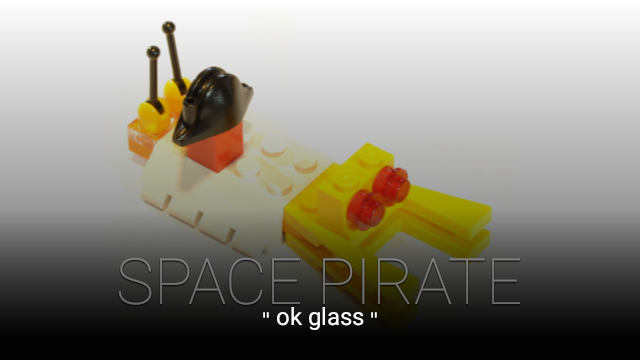
\includegraphics[width=60mm]{images/demoCase/1}}}
		\qquad
		\subfloat[The title slide in the smartphone application.]{{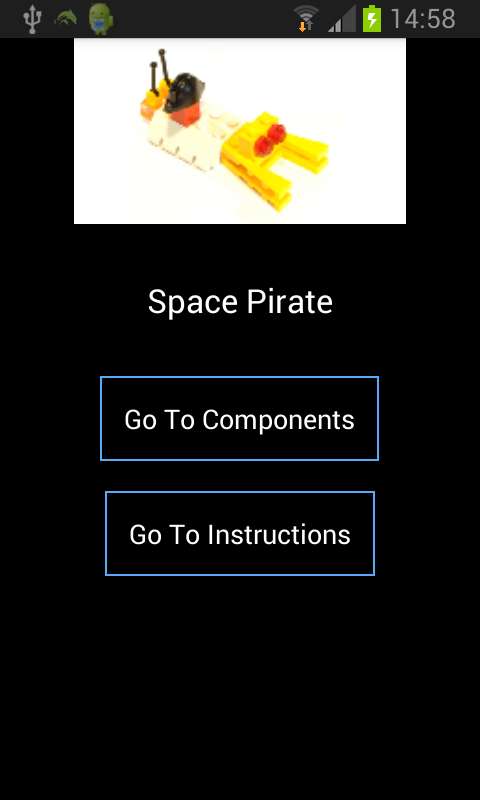
\includegraphics[width=60mm]{images/demoCase/1sp}}}
		\caption{The title slide.}
		\label{demoCase1}
	\end{figure}	

Using the Google Glass application users can, by saying ``ok glass'', bring up the voice command menu, seen in Figure~\ref{demoCaseVoiceCommand}, and navigate through the application. In the smartphone application, no voice commands exist, but users may use the two buttons on the title slide in order to skip through the slides to either the components or the instructions. However, in both the Google Glass application and the smartphone application users can simply swipe, using a finger, to the next slide in line. 

	\begin{figure}[H]%ht!]
		\centering
		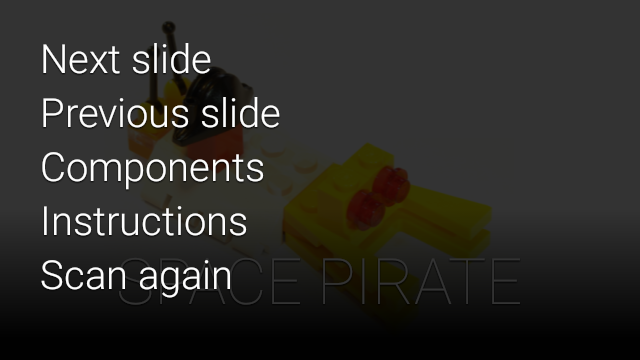
\includegraphics[width=90mm]{images/demoCase/glassVoiceCommand}
		\caption{The voice command menu.}
		\label{demoCaseVoiceCommand}
	\end{figure}


The second slide of the application is the first component slide, seen in Figure~\ref{demoCaseSteering}. Here the user sees the first component needed for assembling the Space Pirate, which is the Steering component, seen in Figure~\ref{demoCaseSteering}~(d). While the Google Glass application is fixed in its layout, the smartphone application can be altered in terms of the screen orientation. This is because while Google Glass is mounted on the user's head and may not be rotated, the smartphone can. As such the smartphone application can be viewed in either portrait orientation mode, seen in Figure~\ref{demoCaseSteering}~(b), or in landscape orientation mode, seen in Figure~\ref{demoCaseSteering}~(c). In both cases the image allocates the same percentage of screen space in width as the image does in the Google Glass application, which is \(\frac{3}{8}\) of the screen. For the remainder of this demonstration walkthrough the screen shots of the smartphone application will be in landscape mode, but it should be noted that all slides in the smartphone application may be viewed in both portrait orientation mode and landscape orientation mode.

	\begin{figure}[H]%ht!]
		\centering
		\subfloat[The first component card.]{{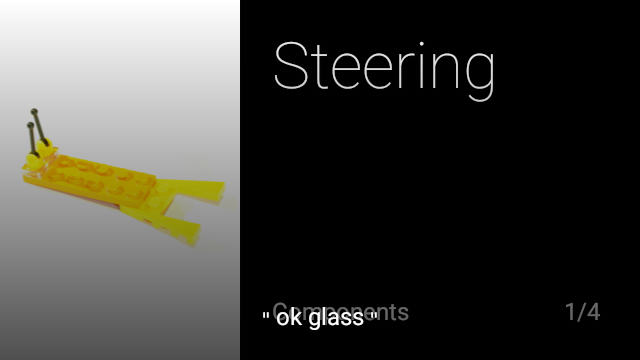
\includegraphics[width=60mm]{images/demoCase/2}}}
		\qquad
		\subfloat[The first component slide in portrait screen orientation.]{{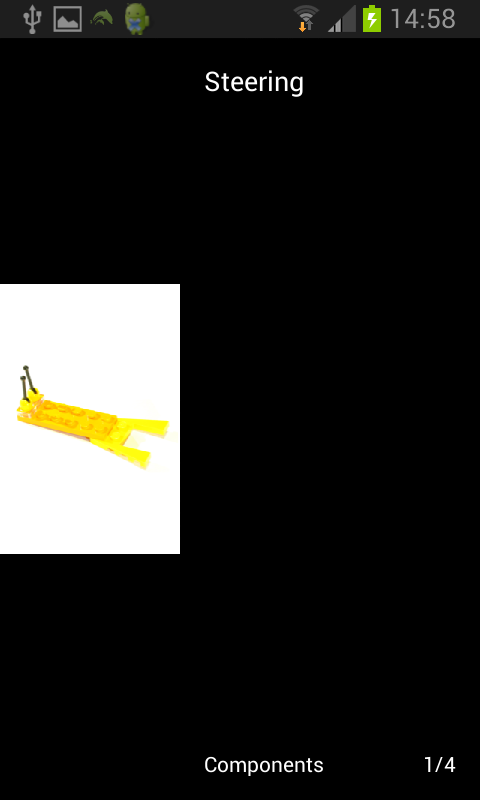
\includegraphics[width=60mm]{images/demoCase/2spP}}}
		\qquad
		\subfloat[The first component slide in landscape screen orientation.]{{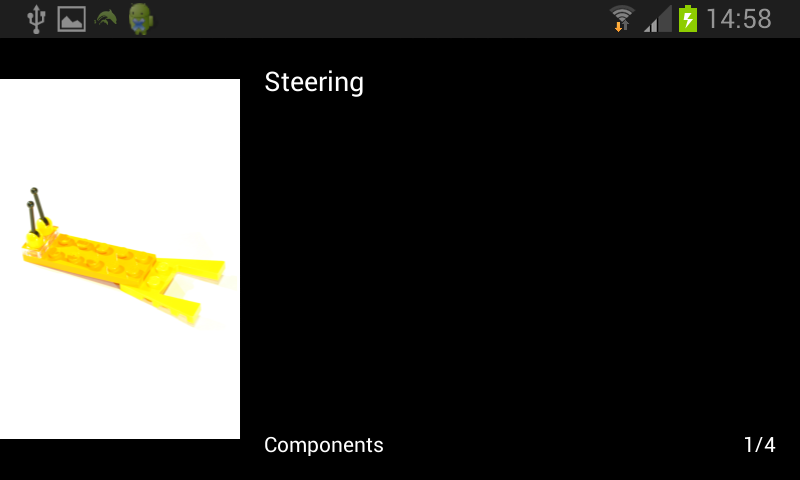
\includegraphics[width=60mm]{images/demoCase/2spL}}}
		\qquad
		\subfloat[The Steering component.]{{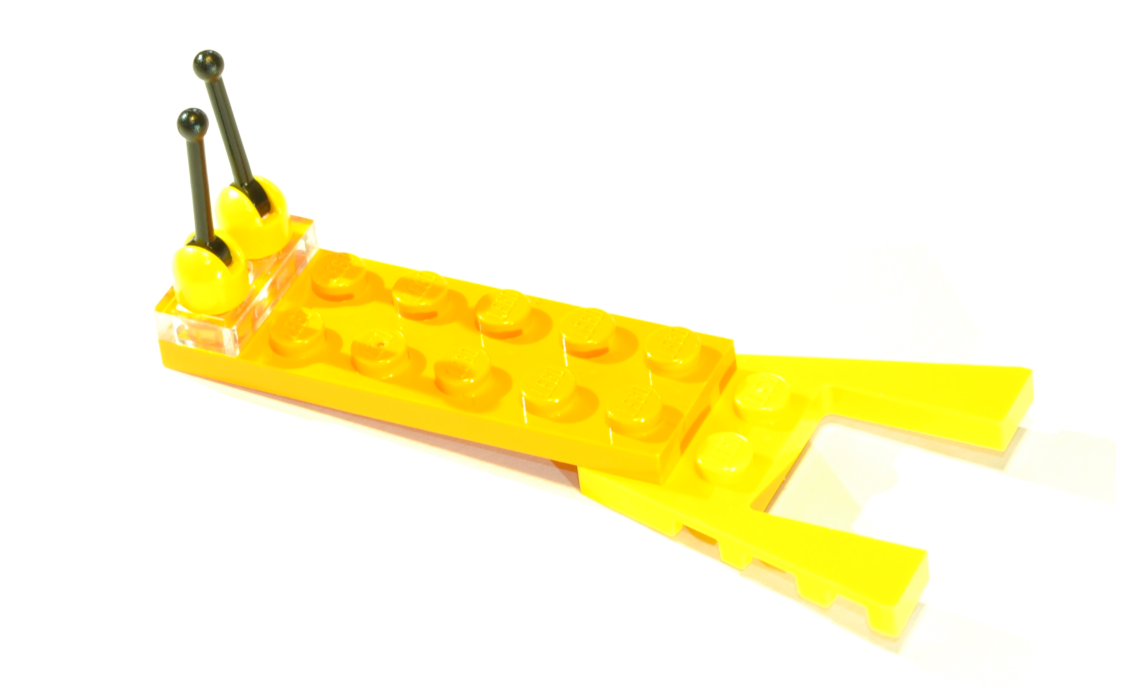
\includegraphics[width=60mm]{images/rawImages/BILD_1}}}
		\caption{The first component.}
		\label{demoCaseSteering}
	\end{figure}

The next slide is the second component slide, seen in Figure~\ref{demoCaseTailLight}, which uses only text to describe the component. The component is called ``Tail Light'', and can be seen in Figure~\ref{demoCaseTailLight}~(c). The reason for not using an image to describe the Tail Light component is because the text was deemed sufficient enough for the user to distinguish the Tail Light component from the others.

	\begin{figure}[ht!]
		\centering
		\subfloat[The second component card.]{{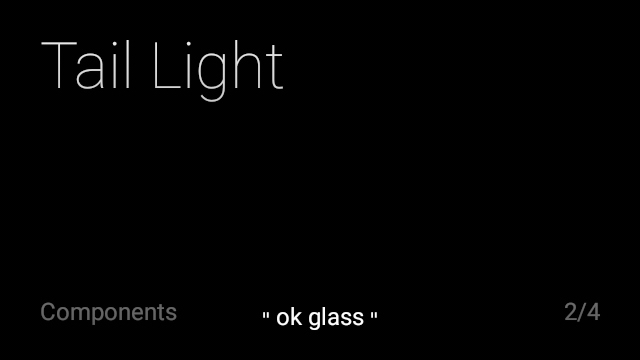
\includegraphics[width=60mm]{images/demoCase/3}}}
		\qquad
		\subfloat[The second component slide.]{{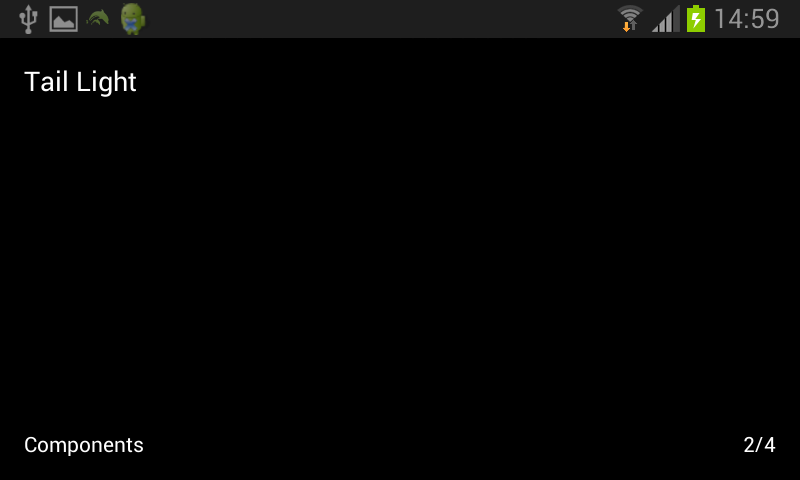
\includegraphics[width=60mm]{images/demoCase/3sp2}}}
		\qquad
		\subfloat[The Tail Light component.]{{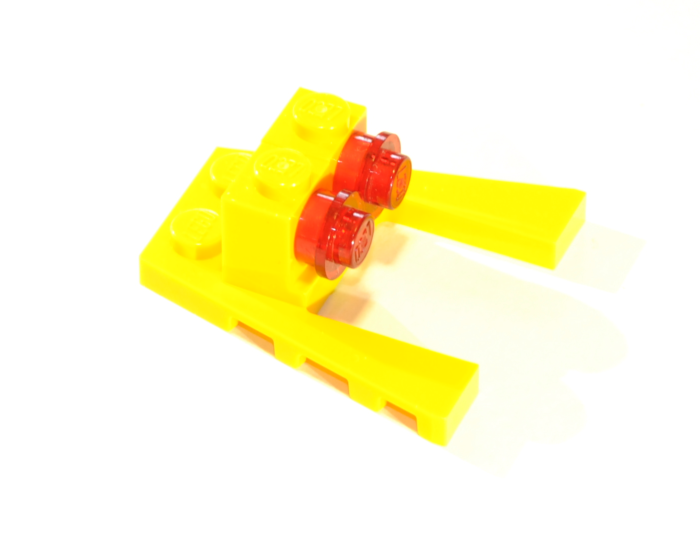
\includegraphics[width=60mm]{images/rawImages/BILD_2}}}
		\caption{The second component.}
		\label{demoCaseTailLight}
	\end{figure}

The fourth slide in the application is the third component slide, seen in Figure~\ref{demoCaseBody}. Similar to the first component slide, the third component slide uses both and image as well as text in order to describe which component the user need. The component is called ``Body'' and can be seen in Figure~\ref{demoCaseBody}~(c). The reason for using both text and an image to describe the Body component is because the component name is a general one and could potentially apply to the Steering component as well.

	\begin{figure}[H]%ht!]
		\centering
		\subfloat[The third component card.]{{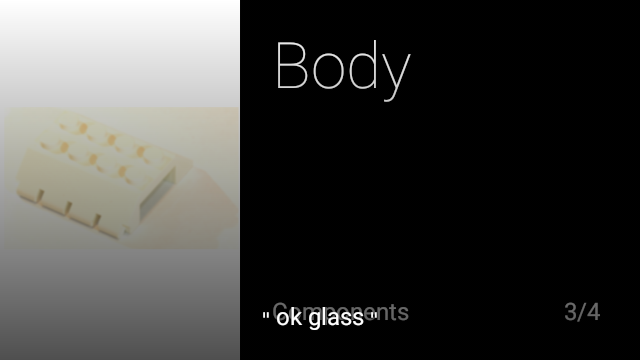
\includegraphics[width=60mm]{images/demoCase/4}}}
		\qquad
		\subfloat[The third component slide.]{{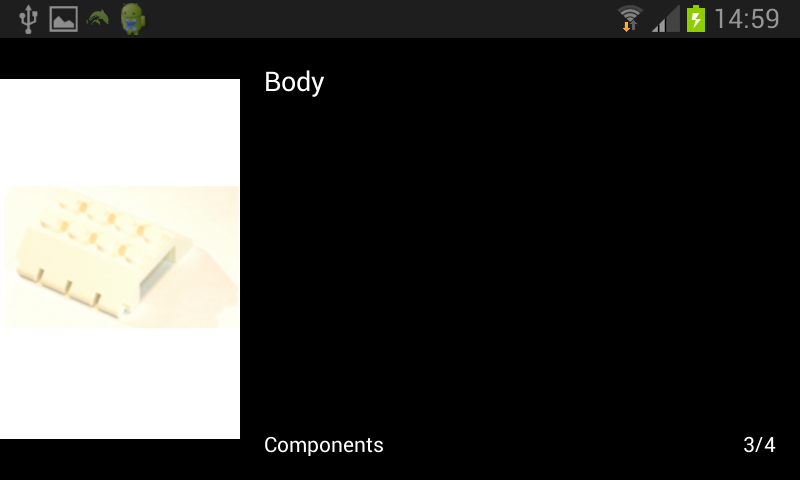
\includegraphics[width=60mm]{images/demoCase/4sp}}}
		\qquad
		\subfloat[The Body component.]{{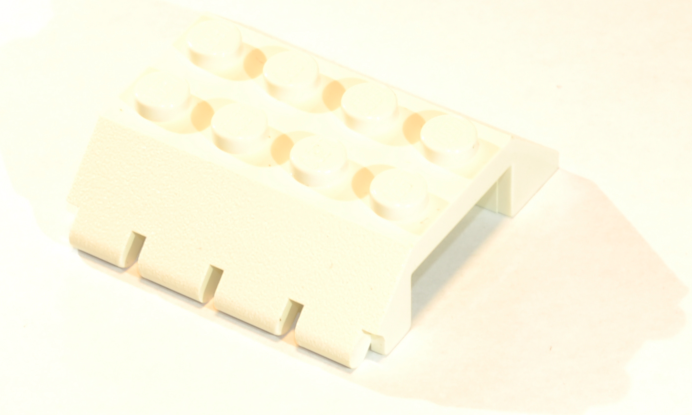
\includegraphics[width=60mm]{images/rawImages/BILD_3}}}
		\caption{The third component.}
		\label{demoCaseBody}
	\end{figure}
	
The next slide is the fourth and last component slide, seen in Figure~\ref{demoCasePirate}. Similar to Figure~\ref{demoCaseTailLight}, the fourth component is also only described in text. The component is called ``Pirate'' and can be seen in Figure~\ref{demoCasePirate}~(c).

	\begin{figure}[H]%ht!]
		\centering
		\subfloat[The fourth component card.]{{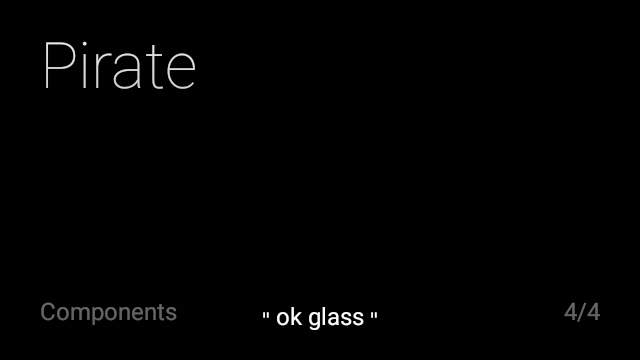
\includegraphics[width=60mm]{images/demoCase/5}}}
		\qquad
		\subfloat[The fourth component slide.]{{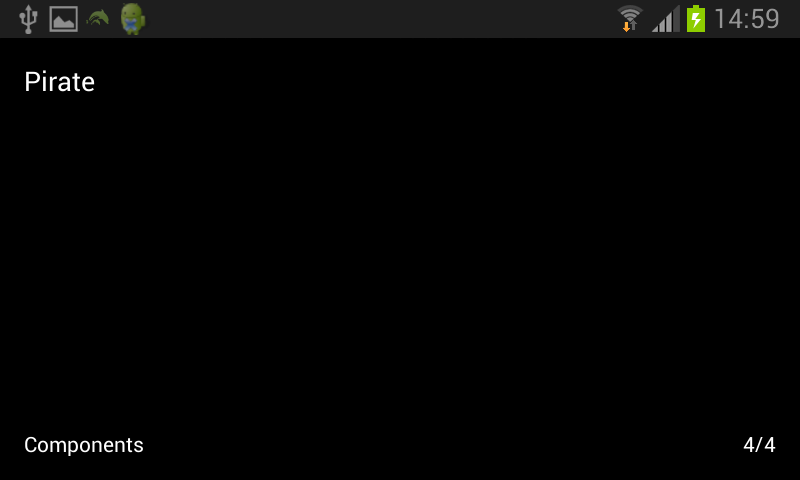
\includegraphics[width=60mm]{images/demoCase/5sp}}}
		\qquad
		\subfloat[The Pirate component.]{{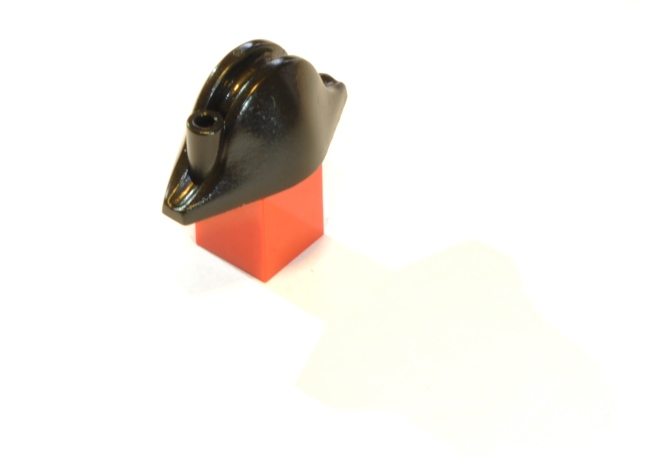
\includegraphics[width=60mm]{images/rawImages/BILD_4}}}
		\caption{The fourth component.}
		\label{demoCasePirate}
	\end{figure}

After the components come the instructions. At this point the user should have gathered all of the components and be ready to assemble the product. The first instruction slide can be seen in Figure~\ref{demoCaseInstruction1}. The goal is to combine the Tail Light component and the Steering component in to what can be seen in Figure~\ref{demoCaseInstruction1}~(c).

	\begin{figure}[H]%ht!]
		\centering
		\subfloat[The first instruction card.]{{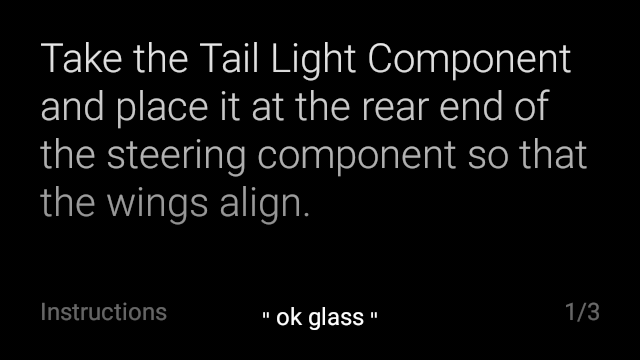
\includegraphics[width=60mm]{images/demoCase/6}}}
		\qquad
		\subfloat[The first instruction slide.]{{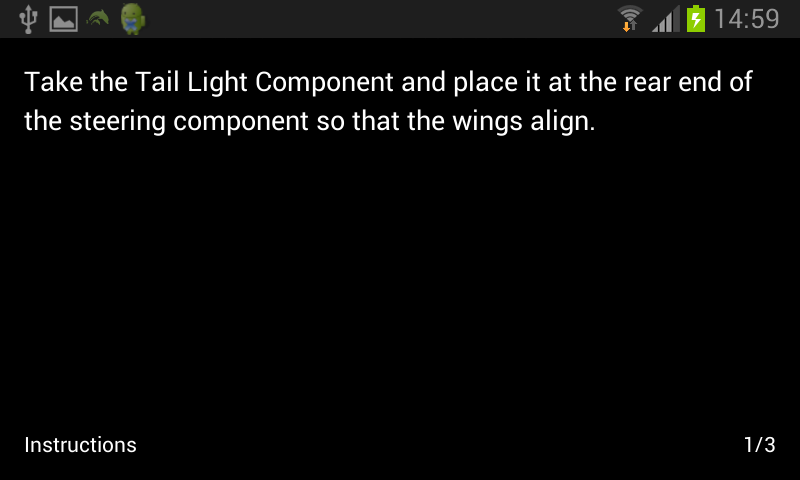
\includegraphics[width=60mm]{images/demoCase/6sp}}}
		\qquad
		\subfloat[The goal of the first instruction.]{{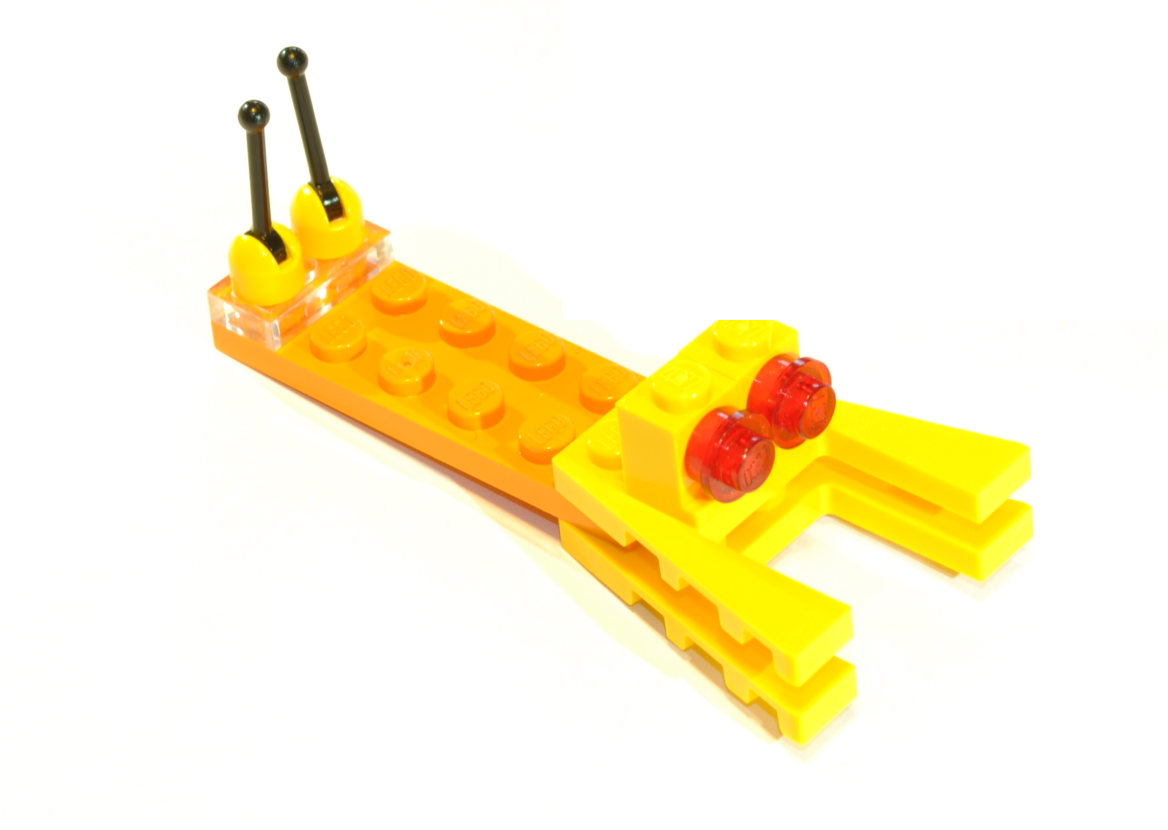
\includegraphics[width=60mm]{images/rawImages/BILD_5}}}
		\caption{The first instruction.}
		\label{demoCaseInstruction1}
	\end{figure}

The second instruction is described with only an image and no text, as seen in Figure~\ref{demoCaseInstruction2}. The reason for this is because the alignment of the components would be difficult to describe in text and a larger image makes it easier for the user to see how the components should fit together. Using both text and an image would mean that the image would be scaled down. The user is, with the instruction, supposed to combine the Body component and the Pirate component in to what can be seen in Figure~\ref{demoCaseInstruction2}~(c).

	\begin{figure}[H]%ht!]
		\centering
		\subfloat[The second instruction card.]{{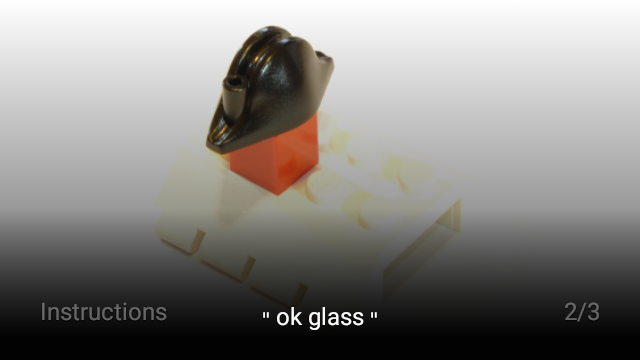
\includegraphics[width=60mm]{images/demoCase/7}}}
		\qquad
		\subfloat[The second instruction slide.]{{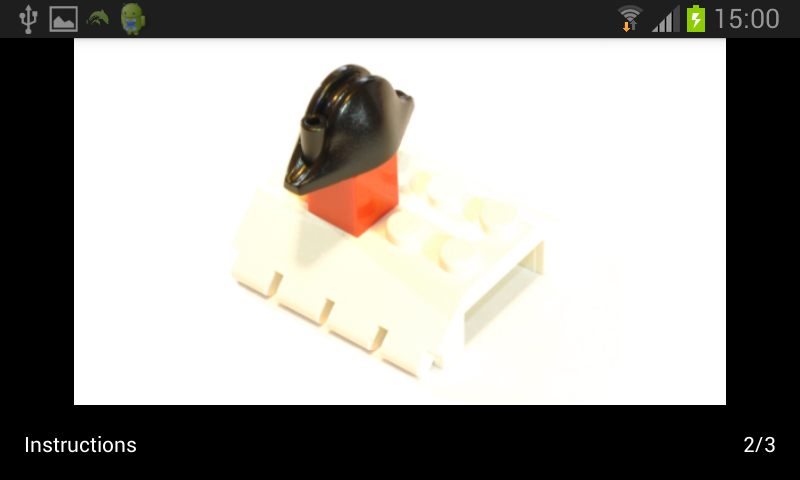
\includegraphics[width=60mm]{images/demoCase/7sp}}}
		\qquad
		\subfloat[The goal of the second instruction.]{{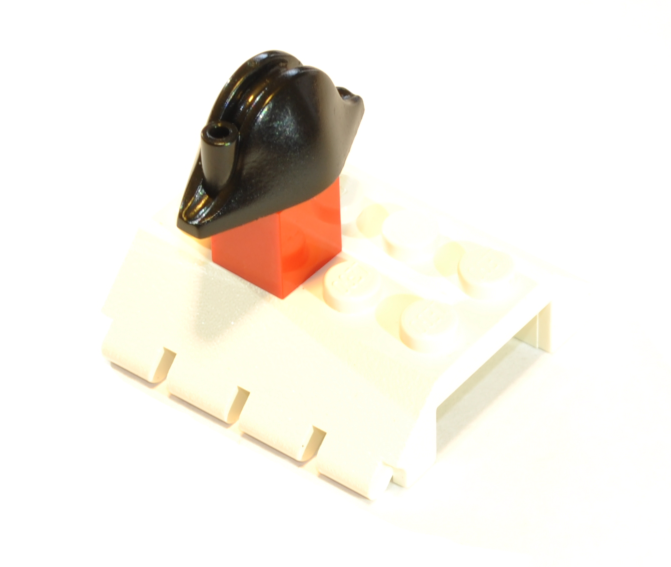
\includegraphics[width=60mm]{images/rawImages/BILD_8}}}
		\caption{The second instruction.}
		\label{demoCaseInstruction2}
	\end{figure}

The final slide, seen in Figure~\ref{demoCaseInstruction3}, describes the final instruction in both text and an image. The reason for using both text and an image is because the text may contain enough information on how to combine the components and the image can be used as visual guideline. Potentially the image could be enough information on its own, and could as such be shown in full scale instead. However, since the image does not need to be full scale it will take up less data space and as such be faster to download compared to a full scale image.

	\begin{figure}[H]%ht!]
		\centering
		\subfloat[The third instruction card.]{{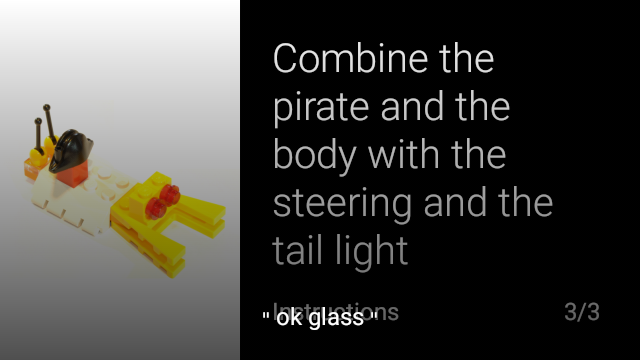
\includegraphics[width=60mm]{images/demoCase/8}}}
		\qquad
		\subfloat[The third instruction slide.]{{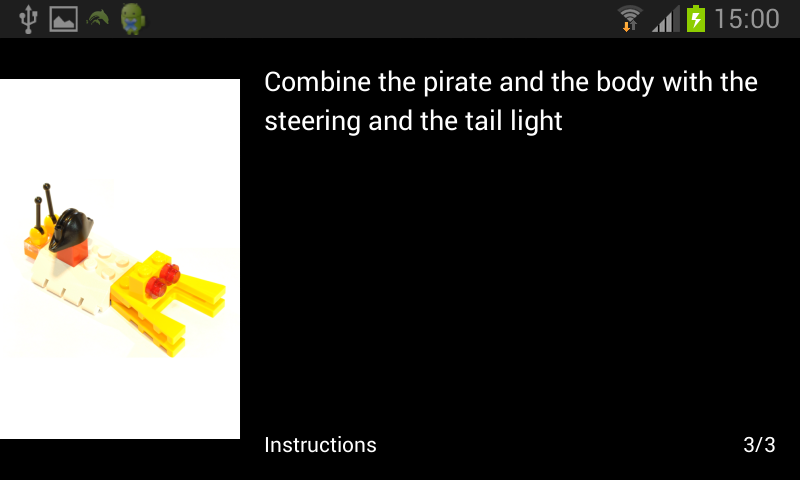
\includegraphics[width=60mm]{images/demoCase/8sp}}}
		\qquad
		\subfloat[The goal of the third instruction.]{{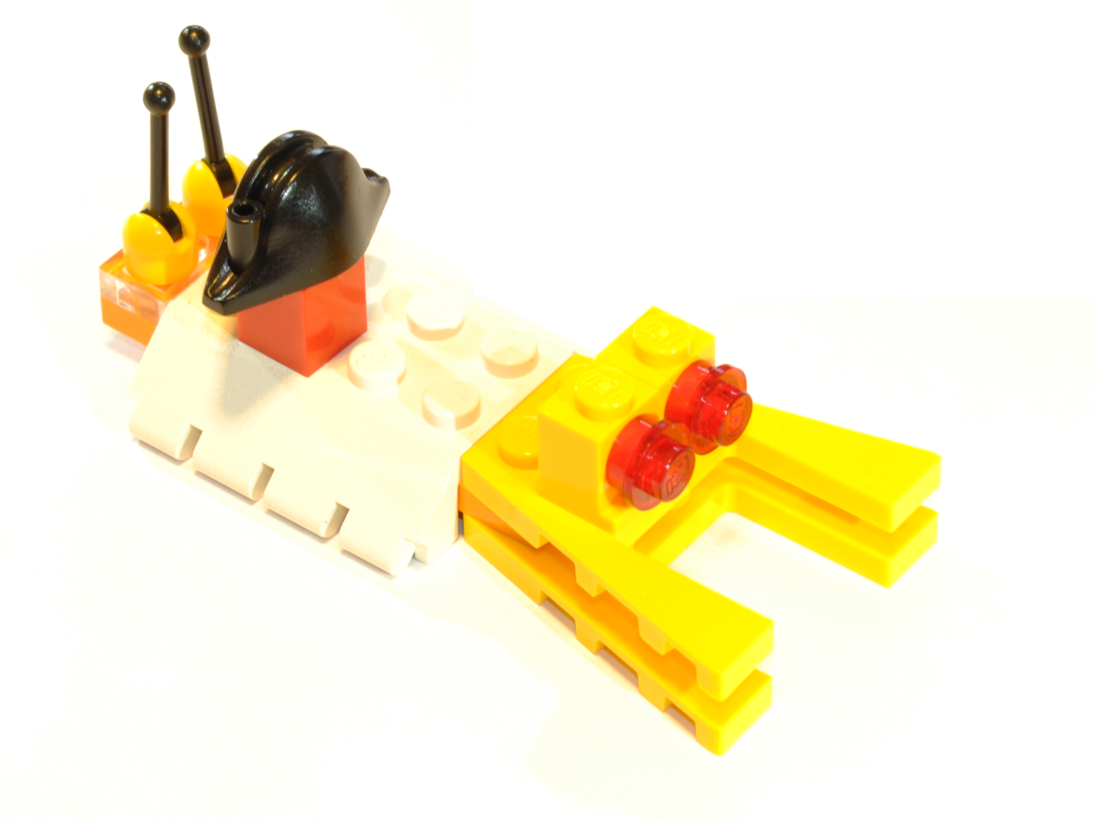
\includegraphics[width=60mm]{images/rawImages/BILD_6}}}
		\caption{The third instruction.}
		\label{demoCaseInstruction3}
	\end{figure}

When the user has completed what the third and last instructions say, the product is fully assembled. As such, the application may now be closed or another QR code may be scanned. In the Google Glass application the user can say ``ok glass'' and then ``Scan again'', in order to bring up the camera and scan another QR code. In the smartphone application the user may press the default back button on the smartphone in order to bring up the camera screen and scan another QR code.
% done

%The following are the results of the tests performed on the application, both on the Google Glass version as well as the smartphone version.

\subsection{Text Length}
The following are the results from evaluating the number of characters that may fit on a card in the Google Glass application, both when using only text and when using both text and an image. The test was performed only once for each device since despite randomising the characters used, the text length would not differ significally from one case to another. As seen in the following results none of the tests resulted in an additional card with only one character. Had that been the case, different combinations of characters may have changed the number of cards necessary to display all of the information. As that is not the case only one test was deemed sufficient enough to determine the number of card required to display the same information as displayed on a smartphone device.

However, some trial and error was part of the process of finding how many characters would fill the smartphone screens. 550 was deemed a suitable number for Samsung Galaxy SII och 750 was deemed a suitable number for Samsung Galaxy SIII, as that many characters filled up the screen and yet still left some room for longer characters or longer words, as seen in Figure~\ref{glassTestTextLengthRaw}. For Samsung Galaxy SII, 600 characters did not fit on the screen, and for Samsung Galaxy SIII, 800 characters did not fit on the screen. As such 550 and 750 respectively was set as the maximum number of characters, although depending on the characters being displayed the text may use up more or less space since an 'i' does not take up as much space as a 'w'. The filled smartphone screens can be seen in Figure~\ref{glassTestTextLengthRaw}.

	\begin{figure}[H]%ht!]
		\centering
    		\subfloat[The Samsung Galaxy SII screen.]{{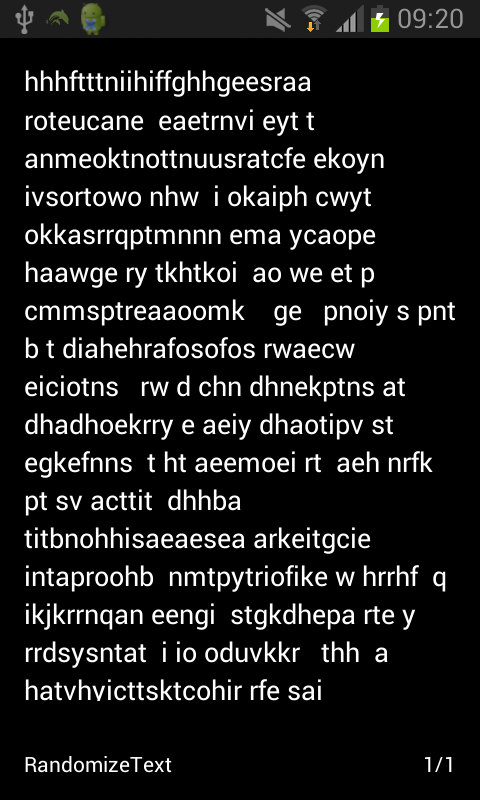
\includegraphics[width=50mm]{images/textLengthTestImages/S2_Raw}}}
   		 \qquad
		\subfloat[The Samsung Galaxy SIII screen.]{{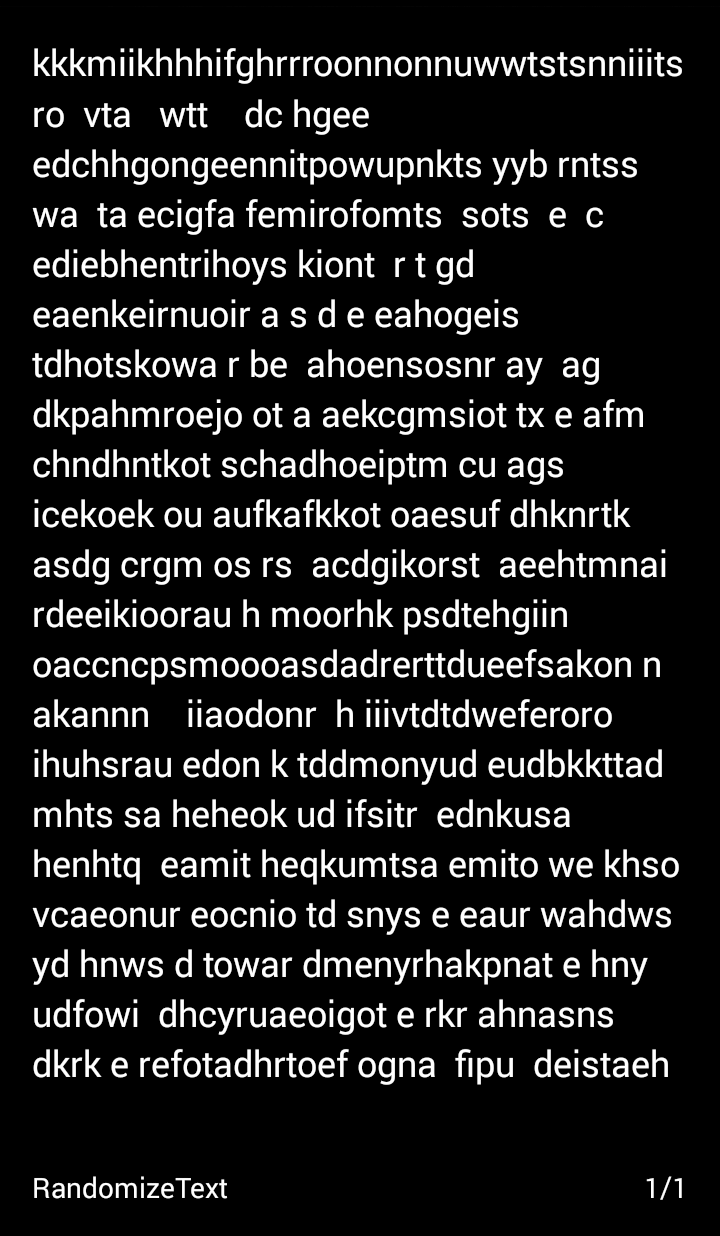
\includegraphics[width=50mm]{images/textLengthTestImages/S3_Raw}}}
   		 \qquad
		\caption{The maximum text length on the smartphone application.}
		\label{glassTestTextLengthRaw}
	\end{figure}

When translating the results from the smartphones to Google Glass the same text was used and simply copied over to the Google Glass application. The result of the text that filled the Samsug Galaxy SIII screen, seen in Figure~\ref{glassTestTextLengthRaw}~(a), can be seen in Figure~\ref{glassTestTextLengthS2Text}. As seen the text that filled the Samsung Galaxy SII screen took up roughly two and a half cards in the Google Glass application. Although the screen is nearly filled in Figure~\ref{glassTestTextLengthS2Text}~(c) the text is dynamically sized depending on the amount of text being displayed. As such the card can be deemed about half full. Table~\ref{tab:glassTestTextLengthS2TextTable} shows the exact number of characters and words on each card, showing that the last card contains about half the number och characters as the other two cards.

	\begin{figure}[H]%ht!]
		\centering
    		\subfloat[The first slide.]{{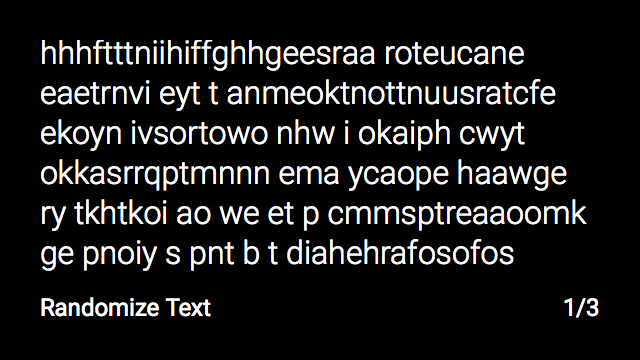
\includegraphics[width=60mm]{images/textLengthTestImages/S2_Text_1}}}
   		 \qquad
		\subfloat[The second slide.]{{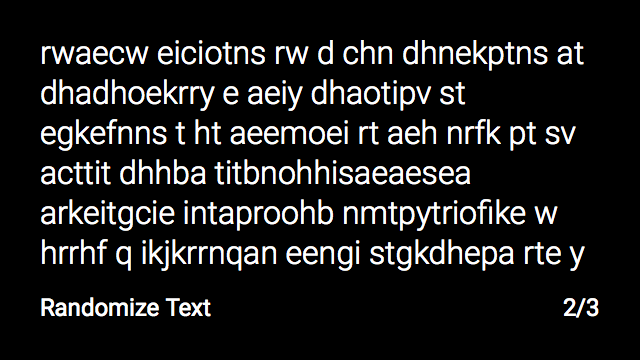
\includegraphics[width=60mm]{images/textLengthTestImages/S2_Text_2}}}
   		 \qquad
		\subfloat[The third slide.]{{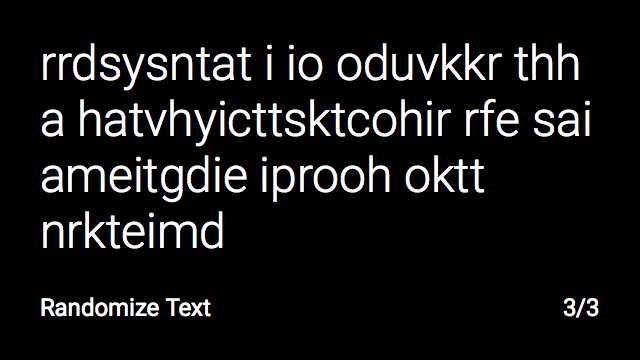
\includegraphics[width=60mm]{images/textLengthTestImages/S2_Text_3}}}
   		 \qquad
		\caption{Samsung Galaxy SII text.}
		\label{glassTestTextLengthS2Text}
	\end{figure}

	\begin{table}[ht!]
    		\caption{Details on text length on Google Glass from Samsung Galaxy SII.} \label{tab:glassTestTextLengthS2TextTable}
		\centering \begin{tabularx}{\textwidth}{l|X|X} \hline
		\textbf{Figure} & \textbf{Number of words} & \textbf{Number of characters} \\ \hline \hline
       
		Figure~\ref{glassTestTextLengthS2Text}~(a)	&30	&229	\\ \hline
		Figure~\ref{glassTestTextLengthS2Text}~(b)	&35	&229	\\ \hline
		Figure~\ref{glassTestTextLengthS2Text}~(c)	&13	&92	\\ \hline
		Figure~\ref{glassTestTextLengthS2Text}~(Total)	&78	&550	\\ \hline
		
		\end{tabularx}
	\end{table}

The result of using the text that filled the Samsung Galaxy SIII screen, seen in Figure~\ref{glassTestTextLengthRaw}~(b), in the Google Glass application can be seen in Figure~\ref{glassTestTextLengthS3Text}. As seen the Samsung Galaxy SIII screen fit more characters than the Samsung Galaxy SII screen and as such three and a half cards in the Google Glass application was needed to display all the text that filled the Samsung Galaxy SIII screen. The exact number of characters and words on each card can be seen in Table~\ref{tab:glassTestTextLengthS3TextTable}.

	\begin{figure}[H]%ht!]
		\centering
    		\subfloat[The first slide.]{{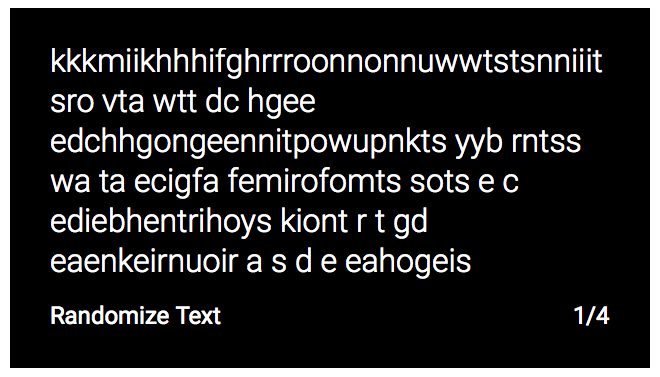
\includegraphics[width=60mm]{images/textLengthTestImages/S3_Text_1}}}
   		 \qquad
		\subfloat[The second slide.]{{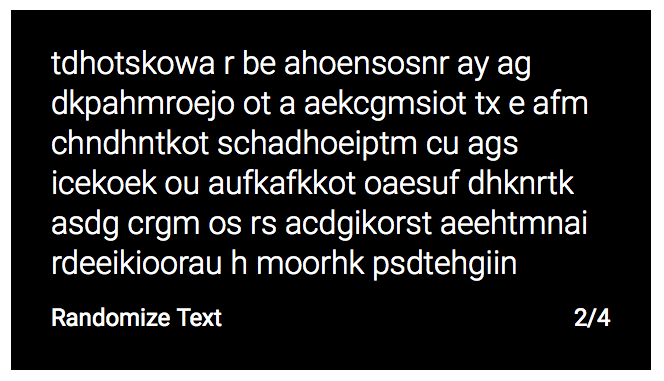
\includegraphics[width=60mm]{images/textLengthTestImages/S3_Text_2}}}
   		 \qquad
		\subfloat[The third slide.]{{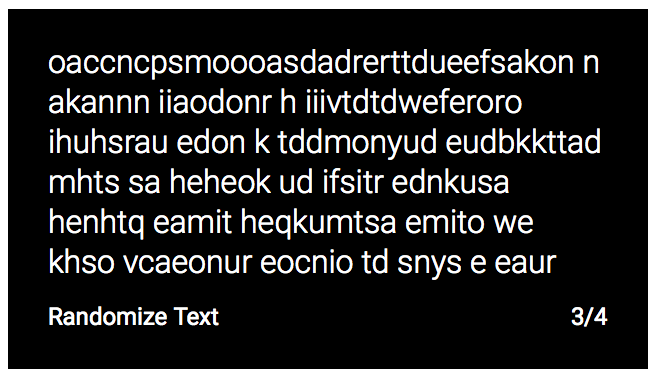
\includegraphics[width=60mm]{images/textLengthTestImages/S3_Text_3}}}
   		 \qquad
		\subfloat[The fourth slide.]{{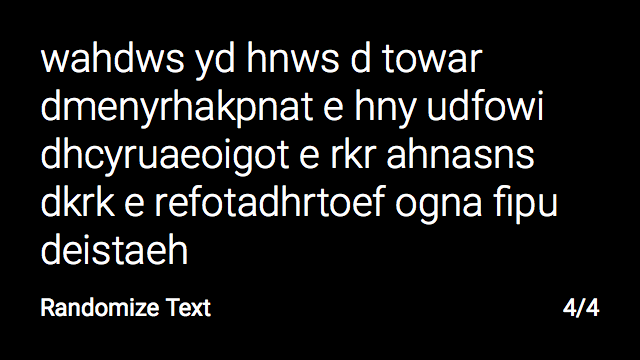
\includegraphics[width=60mm]{images/textLengthTestImages/S3_Text_4}}}
   		 \qquad
		\caption{Samsung Galaxy SIII text.}
		\label{glassTestTextLengthS3Text}
	\end{figure}

	\begin{table}[ht!]
    		\caption{Details on text length on Google Glass from Samsung Galaxy SIII.} \label{tab:glassTestTextLengthS3TextTable}
		\centering \begin{tabularx}{\textwidth}{l|X|X} \hline
		\textbf{Figure} & \textbf{Number of words} & \textbf{Number of characters} \\ \hline \hline
       
		Figure~\ref{glassTestTextLengthS3Text}~(a)	&26	&199	\\ \hline
		Figure~\ref{glassTestTextLengthS3Text}~(b)	&32	&213	\\ \hline
		Figure~\ref{glassTestTextLengthS3Text}~(c)	&29	&217	\\ \hline
		Figure~\ref{glassTestTextLengthS3Text}~(d)	&19	&121	\\ \hline
		Figure~\ref{glassTestTextLengthS3Text}~(Total)	&106	&750	\\ \hline
		
		\end{tabularx}
	\end{table}

Instructions described in text may also be displayed in combination with an image. When text combined with an image is used as the design layout for a slide the maximum number of characters that can be displayed changes. The image, according to Google's predefined card layout design~\cite{glassDesignStyle}, makes up \(3/8\) of the card, and as such the text makes up the other \(5/8\). As such the maximum number of characters can be calculated using the maximum number of characters used when presenting only text.

For Samsung Galaxy SII the maximum number of characters when using both text and an image was calculated as follows: \((5/8)*550~=~343.75\). As three quarters of a character is of no use the maximum number of characters on the Samsung Galaxy SII screen is 343 characters. The result of using the same text as when displaying only text on Samsung Galaxy SII, only shorten down to 343 characters can be seen in Figure~\ref{glassTestTextLengthS2Columns}, with specific numbers in Table~\ref{tab:glassTestTextLengthS2ColumnsTable}.

	\begin{figure}[H]%ht!]
		\centering
		\subfloat[The first slide.]{{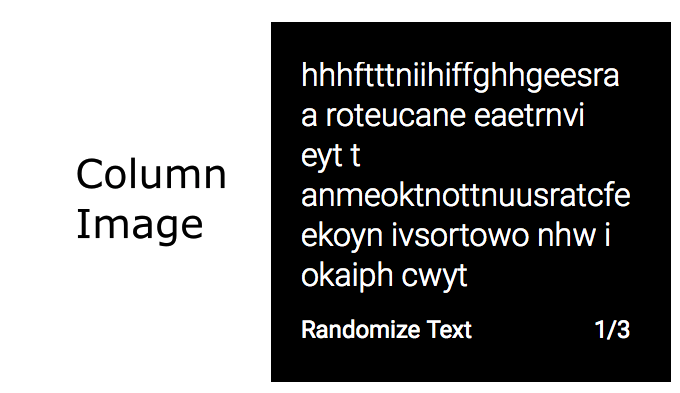
\includegraphics[width=60mm]{images/textLengthTestImages/S2_Columns_1}}}
   		 \qquad
		\subfloat[The second slide.]{{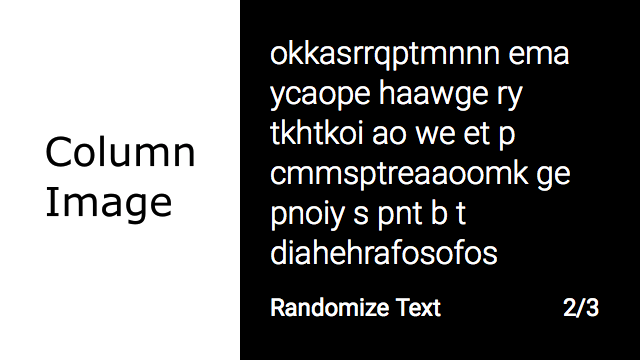
\includegraphics[width=60mm]{images/textLengthTestImages/S2_Columns_2}}}
   		 \qquad
		\subfloat[The third slide.]{{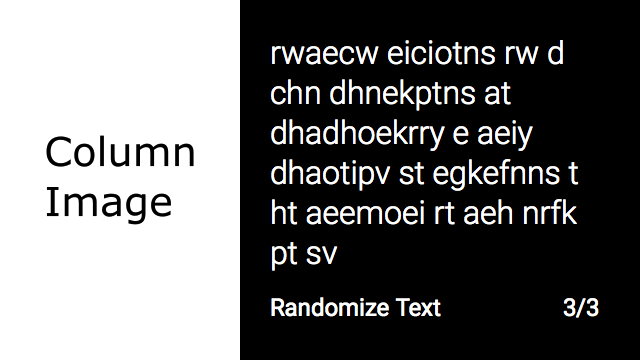
\includegraphics[width=60mm]{images/textLengthTestImages/S2_Columns_3}}}
   		 \qquad
		\caption{Samsung Galaxy SII text and image.}
		\label{glassTestTextLengthS2Columns}
	\end{figure}

	\begin{table}[ht!]
    		\caption{Details on text length on Google Glass from Samsung Galaxy SII.} \label{tab:glassTestTextLengthS2ColumnsTable}
		\centering \begin{tabularx}{\textwidth}{l|X|X} \hline
		\textbf{Figure} & \textbf{Number of words} & \textbf{Number of characters} \\ \hline \hline
       
		Figure~\ref{glassTestTextLengthS2Columns}~(a)	&12	&118	\\ \hline
		Figure~\ref{glassTestTextLengthS2Columns}~(b)	&18	&111	\\ \hline
		Figure~\ref{glassTestTextLengthS2Columns}~(c)	&21	&114	\\ \hline
		Figure~\ref{glassTestTextLengthS2Columns}~(Total)	&51	&343	\\ \hline
		
		\end{tabularx}
	\end{table}

The maximum number of characters when using both text and and image on Samsung Galaxy SIII was calculated the same way as for Samsung Galaxy SII, as follows: \((5/8~=~468.75)\). As three quarters of a character is of no use the maximum number of characters when displaying both text and an image is as such 468 characters. The result of using the same text as in Figure~\ref{glassTestTextLengthRaw}, only shorten down to 468 characters, in the Google Glass application can be seen in Figure~\ref{glassTestTextLengthS3Columns}. The application requires about three and a half card to be able to display all of the text. The exact number of characters and words on each card can be fount in Table~\ref{tab:glassTestTextLengthS3ColumnsTable}.

	\begin{figure}[H]%ht!]
		\centering
    		\subfloat[The first slide.]{{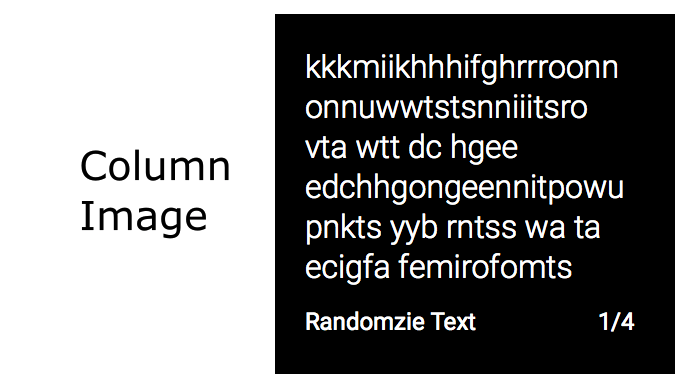
\includegraphics[width=60mm]{images/textLengthTestImages/S3_Columns_1}}}
   		 \qquad
		\subfloat[The second slide.]{{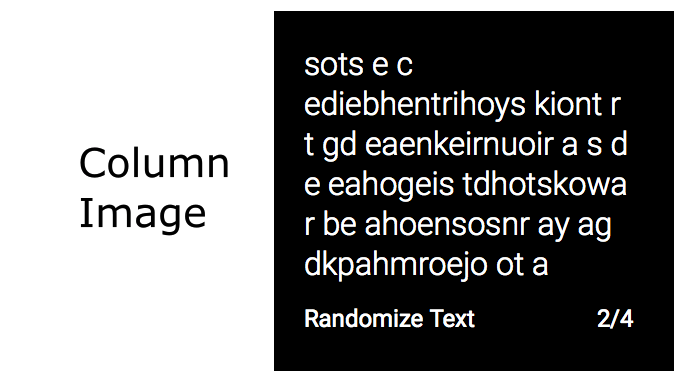
\includegraphics[width=60mm]{images/textLengthTestImages/S3_Columns_2}}}
   		 \qquad
		\subfloat[The third slide.]{{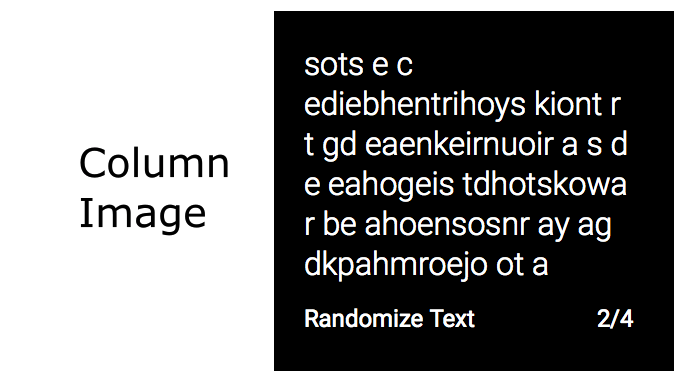
\includegraphics[width=60mm]{images/textLengthTestImages/S3_Columns_2}}}
   		 \qquad
		\subfloat[The fourth slide.]{{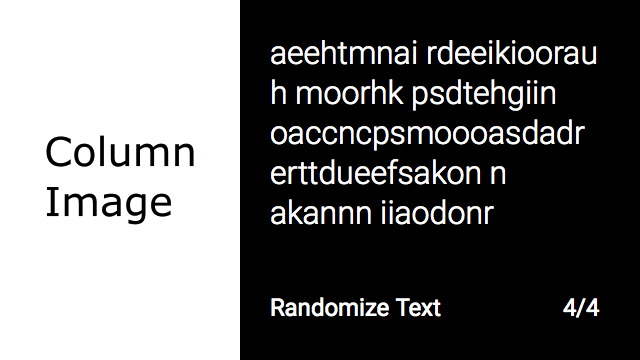
\includegraphics[width=60mm]{images/textLengthTestImages/S3_Columns_4}}}
   		 \qquad
		\caption{Samsung Galaxy SIII text and image.}
		\label{glassTestTextLengthS3Columns}
	\end{figure}

	\begin{table}[ht!]
    		\caption{Details on text length on Google Glass from Samsung Galaxy SIII.} \label{tab:glassTestTextLengthS3ColumnsTable}
		\centering \begin{tabularx}{\textwidth}{l|X|X} \hline
		\textbf{Figure} & \textbf{Number of words} & \textbf{Number of characters} \\ \hline \hline
       
		Figure~\ref{glassTestTextLengthS3Columns}~(a)	&12	&127	\\ \hline
		Figure~\ref{glassTestTextLengthS3Columns}~(b)	&23	&124	\\ \hline
		Figure~\ref{glassTestTextLengthS3Columns}~(c)	&18	&115	\\ \hline
		Figure~\ref{glassTestTextLengthS3Columns}~(d)	&9	&102	\\ \hline
		Figure~\ref{glassTestTextLengthS3Columns}~(Total)	&62	&468	\\ \hline
		
		\end{tabularx}
	\end{table}

Overall a slide in the Google Glass application, which contains only text, can fit around 200 characters, which corresponds to somewhere between 25 to 30 words. When using both text and and image the number of characters that may fit on a slide in the Google Glass application is about 115, which corresponds to about 15 words. In total the Google Glass application requires 3 to 4 cards for every slide in the smartphone application, depending on the size of the smartphone screen, in order to display the same text as a full slide in the smartphone application.

\subsection{Distance to the QR Code}

In Table~\ref{tab:distanceAverage} the average time for registering and decoding a QR code while varying the distance to the QR code can be seen. The size of the QR code was optimised for a distance of two decimeters between the QR code and the device, which also shows in the results as all devices registered the QR code fastest at a distance of two decimeters. The QR code used encoded only one character, an 'a'. The results from every individual run can be seen in Appendix~\ref{app:results}

	\begin{table}[H]%ht!]
    		\caption{Average time of registering a QR code with varying distance.} \label{tab:distanceAverage}
		\centering \begin{tabularx}{\textwidth}{X|X|X|X} \hline
		\textbf{Distance (decimeter(s))} & \textbf{Google Glass (sec)} & \textbf{Samsung Galaxy SII (sec)} & \textbf{Samsung Galaxy SIII (sec)} \\ \hline \hline
       
		1.0	&1.919976807	&1.965959850	&1.839656134	\\ \hline
		2.0	&1.831889852	&1.649790392	&1.487449920	\\ \hline
		3.0	&2.227158610	&1.921767210	&1.568837591	\\ \hline
		
		\end{tabularx}
	\end{table}

\subsection{Complexity of the QR Code}

Table~\ref{tab:complexityAverage} shows the average time for each device to both register and decode a QR code of varying complexity. The distance to the QR codes where two decimeters, as the size of the QR code was optimised for a distance of two decimeters between the QR code and the device. As seen in Table~\ref{tab:complexityAverage} some of the results are infinite, meaning that the device was never able to register the QR code due to the high complexity of the QR code. Samsung Galaxy SIII was able to both register and decode all three of the QR codes, Samsung Galaxy SII was not able to decode the most complex QR code and Google Glass was only able to register the simplest QR code.

One explanation as to why Google Glass was not able to register any QR code other than the simplest one would be that the Google Glass camera did not auto focus as well as both Samsung Galaxy SII and Samsung Galaxy SIII. As such the complexity of the QR code made it difficult to register the QR code. The difference can be seen in Figure~\ref{glassDemoQR}. Every single test run for each device can be found in Appendix~\ref{app:results}.

	\begin{table}[H]%ht!]
    		\caption{Average time of registering a QR code with varying density.} \label{tab:complexityAverage}
		\centering \begin{tabularx}{\textwidth}{l|X|X|X} \hline
		\textbf{Encoded Characters} & \textbf{Google Glass (sec)} & \textbf{Samsung Galaxy SII (sec)} & \textbf{Samsung Galaxy SIII (sec)} \\ \hline \hline
       
		1	&1.831889852	&1.649790392	&1.487449920	\\ \hline
		50	&\textit{Infinite}	&2.096434673	&1.913361687	\\ \hline
		100	&\textit{Infinite}	&\textit{Infinite}	&1.949743816	\\ \hline
		
		\end{tabularx}
	\end{table}

\subsection{Display Time}

The average display time of each device, with varying information sizes, can be seen in Table~\ref{tab:averageDisplaySpeedGoogleGlass}. As the size of the information increased, so did the average display time. The increase in time came as a result of all information being downloaded at the same time, and is then handled by the device. Although only the currently visible information is sent to the display, there is still more information handled by the device and as such the device must search through more information in order to determine which information is to be displayed. 

The display time is also affected by other background processes running at the same time. The average display time also only shows the time from when the information was sorted into classes until the information was sent to the display, and as such does not take in to account the potential delay the display might add in order to actually display the information to the user. Every single test run for each device can be found in Appendix~\ref{app:results}.

	\begin{table}[ht!]
    		\caption{Average display time for Google Glass with varying information size.} \label{tab:averageDisplaySpeedGoogleGlass}
		\centering \begin{tabularx}{\textwidth}{l|X|X|X} \hline
		\textbf{Information Size (Bytes)} & \textbf{Google Glass (sec)}  & \textbf{Samsung Galaxy SII (sec)}  & \textbf{Samsung Galaxy SIII (sec)} \\ \hline \hline
       
		1 000	&0.310802205	&0.008374156	&0.025498950	 \\ \hline
		100 000 	&0.442440796	&0.020444892	&0.034109654	 \\ \hline
		1 000 000	&0.582170613	&0.050938751	&0.078170083	 \\ \hline

		\end{tabularx}
	\end{table}

\subsection{Summary}
While the Google Glass application and the smartphone application essentially has the same functionality, there are some differences between the two. The Google Glass application may be controlled using voice commands, which is a feature the smartphone application does not have. Otherwise both of the application follows Google's design guidelines in terms of being easy to use and both the Google Glass application and the smartphone application focuses on what is important in the application, which is to scan a QR code and view product information.

Looking at the amount of text which may fit the screen on the different devices, it was shown that a full screen of text on Samsung Galaxy SII covered about two and a half screens on Google Glass. When filling up an entire screen on Samsung Galaxy SIII, the same amount of text filled up about three and a half screens on Google Glass. In other words is the amount of information that may be displayed on Google Glass very limited compared to smartphone devices.

In terms of the other test results it can be seen that the Google Glass application is almost always slower that the smartphone application, on both the Samsung Galaxy SII and the Samsung Galaxy SIII. Google Glass was only about 0.4 seconds behind Samsung Galaxy SII when scanning the QR code from different distances.

However, when the complexity of the QR code was varied, Google Glass had a harder time. While Samsung Galaxy SII was not able to scan and decode the QR code which encoded 100 characters, Google Glass was not even able to scan and decode the QR code which encoded 50 characters. Samsung Galaxy SIII managed to scan and decode all the different QR codes, although the more complex QR codes took about half a second longer to scan and decode.

The display time test was the test where Google Glass fell behind the most. Both Samsung Galaxy SII and Samsung Galaxy SIII manage to send to information to the display in under 0.1 seconds, no matter even though the information size was 1 MB. Google Glass, however, always took longer than 0.1 seconds, even when the information size was only 1 kB.

%%o   Introduction - Summarise your main results
%%o   Give details of the results
%%o   Best presentation? (text, tables, diagrams?)
%o   Implementation Evaluation - your results against your expectations%
%%o   Summary - for this chapter

%\subsection{The Application}

%\subsubsection{Google Glass}

%\subsubsection{Smartphone}

%\subsection{Test Cases}

%\subsubsection{Text Length}

%\subsubsection{Image Size}

%\subsubsection{Comparing Text and Images}

%\subsubsection{Download Speed}

%\subsubsection{Interaction Delay}

%\subsubsection{Background Noise}

%\subsubsection{Size of QR Code}

%\subsubsection{Complexity of QR Code}

%\subsubsection{``Tap Counter''}

%\subsubsection{User Experience}

%\subsubsection{Multitasking}

%\subsubsection{Battery}

%\subsubsection{Connected to Mobile Device}

%\subsubsection{Overall Conclusions}